% Drawing 119/08-7 -- folder 119, batch 08, archive page 156 (PDF page 157).
% Transcription: un carré raturé, puis un carré à deux diagonales
% Kind: struck square, then a square with two diagonals. Method 2 (schematic redraw from the facsimile). Status: ok.
% Notes: A square covered with crossing-out strokes (drawn grey), then a square with both diagonals heavy.
% Coordinates: 1 unit = 1 mm = 1/100 of the crop width (bbox in page fractions: [0.23, 0.42, 0.37, 0.48]).
% Redrawn by Claude (claude-opus-5-5), issue #73, 2026-11-07; not checked by a human; not compiled (no TeX in the session).
% Rights: reproduces part of the work -- behind RENDER_TRANSCRIPTS, never published by itself.
\documentclass[tikz,border=3pt]{standalone}
\usepackage{amsmath,amssymb}
\usetikzlibrary{patterns,arrows.meta}
\tikzset{pencil/.style={black!45}, struck/.style={black!35}, mark/.style={circle,draw,inner sep=1.3pt}, pt/.style={circle,fill,inner sep=0.9pt}, opt/.style={circle,draw,fill=white,inner sep=1.1pt}}
\begin{document}
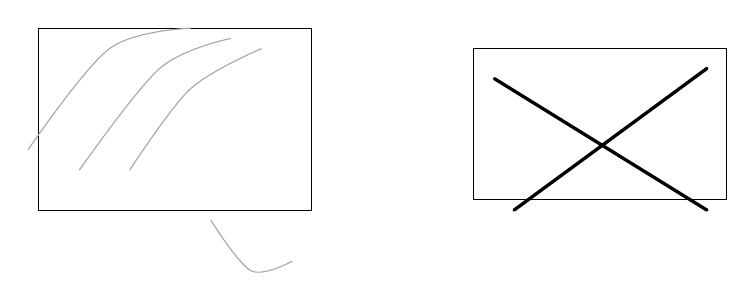
\begin{tikzpicture}[x=1mm,y=1mm,line cap=round,line join=round,font=\scriptsize]
\draw (6.7,-10.3) -- (41.4,-10.3) -- (41.4,-33.4) -- (6.7,-33.4) -- cycle;
\draw[struck] plot[smooth, tension=0.55] coordinates {(5.4,-25.7) (15.7,-12.9) (26,-10.3)};
\draw[struck] plot[smooth, tension=0.55] coordinates {(11.9,-28.3) (22.1,-15.4) (31.1,-11.6)};
\draw[struck] plot[smooth, tension=0.55] coordinates {(18.3,-28.3) (26,-18) (35,-12.9)};
\draw[struck] plot[smooth, tension=0.55] coordinates {(28.6,-34.7) (33.7,-41.1) (38.9,-39.9)};
\draw (62,-12.9) -- (94.1,-12.9) -- (94.1,-32.1) -- (62,-32.1) -- cycle;
\draw[very thick] (64.6,-16.7) -- (91.6,-33.4);
\draw[very thick] (67.1,-33.4) -- (91.6,-15.4);
\end{tikzpicture}
\end{document}
